% With INS the position error grows cubically with time, due to the signal to noise ratio inherent to MEMS IMU sensors \cite{Harle2013}. To compensate for this error, it is preferable that the IMU sensor is mounted on the foot, as will be explained in \cref{sec:INS}. This placement requirement may limit usability. \\

%One advantage of the SHS implementation is that the position error is proportional to the number of steps taken, but without the preference of using foot-based sensors, allowing for other sensor placements \cite{Diez2018b}.

% This section will outline the different PDR methods and focus on an SHS approach to indoor localization.

\chapter{Related Work}
\label{sec:relevant_research}
The person focused indoor localization technique that uses MEMS IMU sensors is called inertial Pedestrian Dead Reckoning (PDR). Dead reckoning indicates that the output of the system will be the relative position change from a starting point \cite{Yu2018}. Within PDR there are two methods, namely Inertial Navigation Systems (INSs) and Step and Heading Systems (SHSs). The INS mechanism integrates the IMU signals directly and is the implementation used most often within research \cite{Diez2018b}. SHS is based on integrating the displacement vectors associated with each step taken during pedestrian locomotion \cite{Davidson2017}.  \par

\section{Inertial Navigation System}
\label{sec:INS}
\begin{figure}[H]
	\centering
	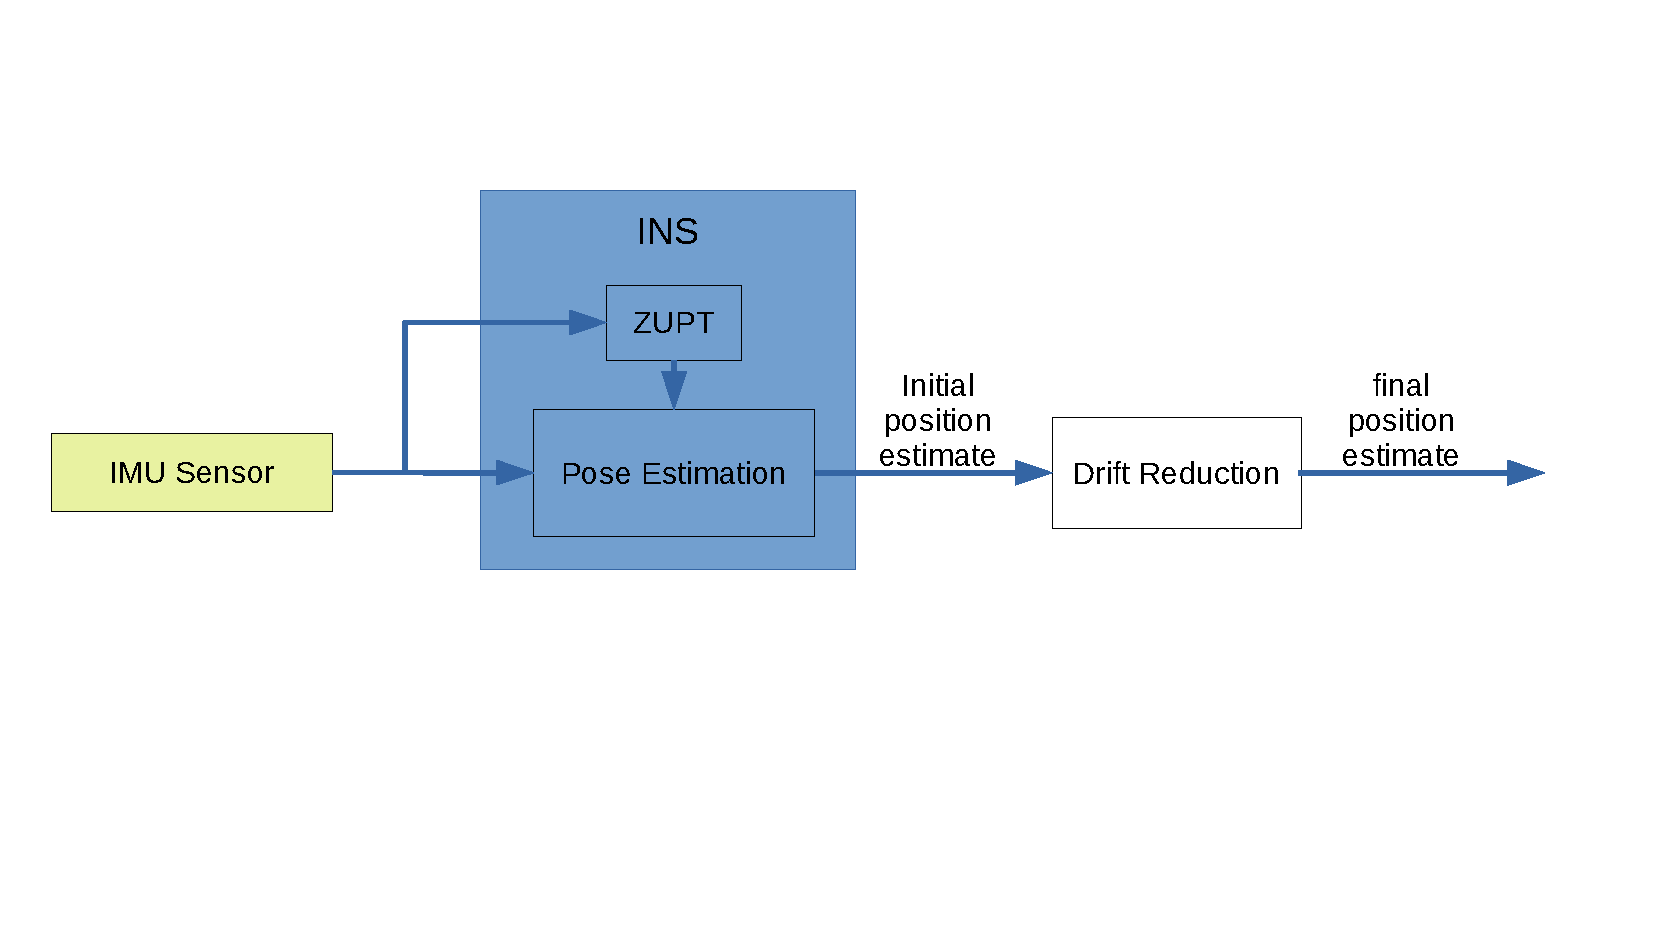
\includegraphics[trim=20 140 290 80, clip, width=0.8\linewidth]{images/INS_diagram}
	\caption{\ac{INS} pedestrian dead reckoning}
	\label{fig:ins_diagram}
\end{figure}
An Inertial Navigation System, as seen in \cref{fig:ins_diagram}, estimates pose, consisting of orientation and position, using sensor fusion algorithms. These methods are directly applied to the signals generated by MEMS IMU sensors \cite{Wu2019}. Examples of sensor fusion algorithms are the Extended Kalman Filter (EKF) and Complementary Filter (CF) \cite{Kok2017}. Sensor fusion algorithms can estimate position and orientation by integrating acceleration twice and integrating angular velocity once, respectively. This integration, in combination with the effects of noise and bias found in MEMS IMU, causes estimation errors to grow cubically with time for INS \cite{Harle2013}. \par

A technique frequently used to compensate for the built-up error in INS is zero velocity update (ZUPT) and zero angular update (ZARU) \cite{Harle2013}. It utilizes the ability to detect time periods in which the sensor is stationary during locomotion. Once detected, ZUPT uses the assumption that speed and angular velocity are zero at that time moment \cite{Wu2019,Harle2013}. this a form of pseudo-measurement. This is because the stationary phase is detected, with zero angular and linear velocity being implied by the assumption, which is not an actual measurement. Comparing the assumption with the output of the sensor fusion algorithm, an error can be calculated and used to compensate for the sensor fusion estimate. This process is generally known as a measurement update and can occur every time a stationary period is detected.  Through this form of measurement update the error grows linearly with number of steps \cite{foxlin2005pedestrian}.\par

Detecting brief stationary time periods in pedestrian IMU data is done easiest when the sensor is placed on the foot \cite{Diez2018,Davidson2017}. This is because a stationary period is much more pronounced in accelerometer data when the sensor is placed there \cite{Yu2019,Wu2019}.  When walking, a foot periodically returns to an actual stationary state and stays there for a brief period of time, approximately 0.1 to 0.3 seconds \cite{Ren2016a}. This has lead to most \ac{INS} research being foot-sensor based \cite{Diez2018,Wu2019}. A recent deviation from this trend, \citet{Solin2018a} overcome this preference for a foot-based system with a combination of several different pseudo measurements, loop closure, and position fixes, opening up new possibilities for implementing INS in non foot based use cases.\\
%The highest accuracy in PDR has been reached with INS in combination with ZUPT \cite{Hardegger2012}.

% Considering this, a focus will be put on implementing a SHS with the potential to handle different carrying modes.
\section{Step and Heading System}
\label{sec:rw-SHS}
\begin{figure}[H]
	\centering
	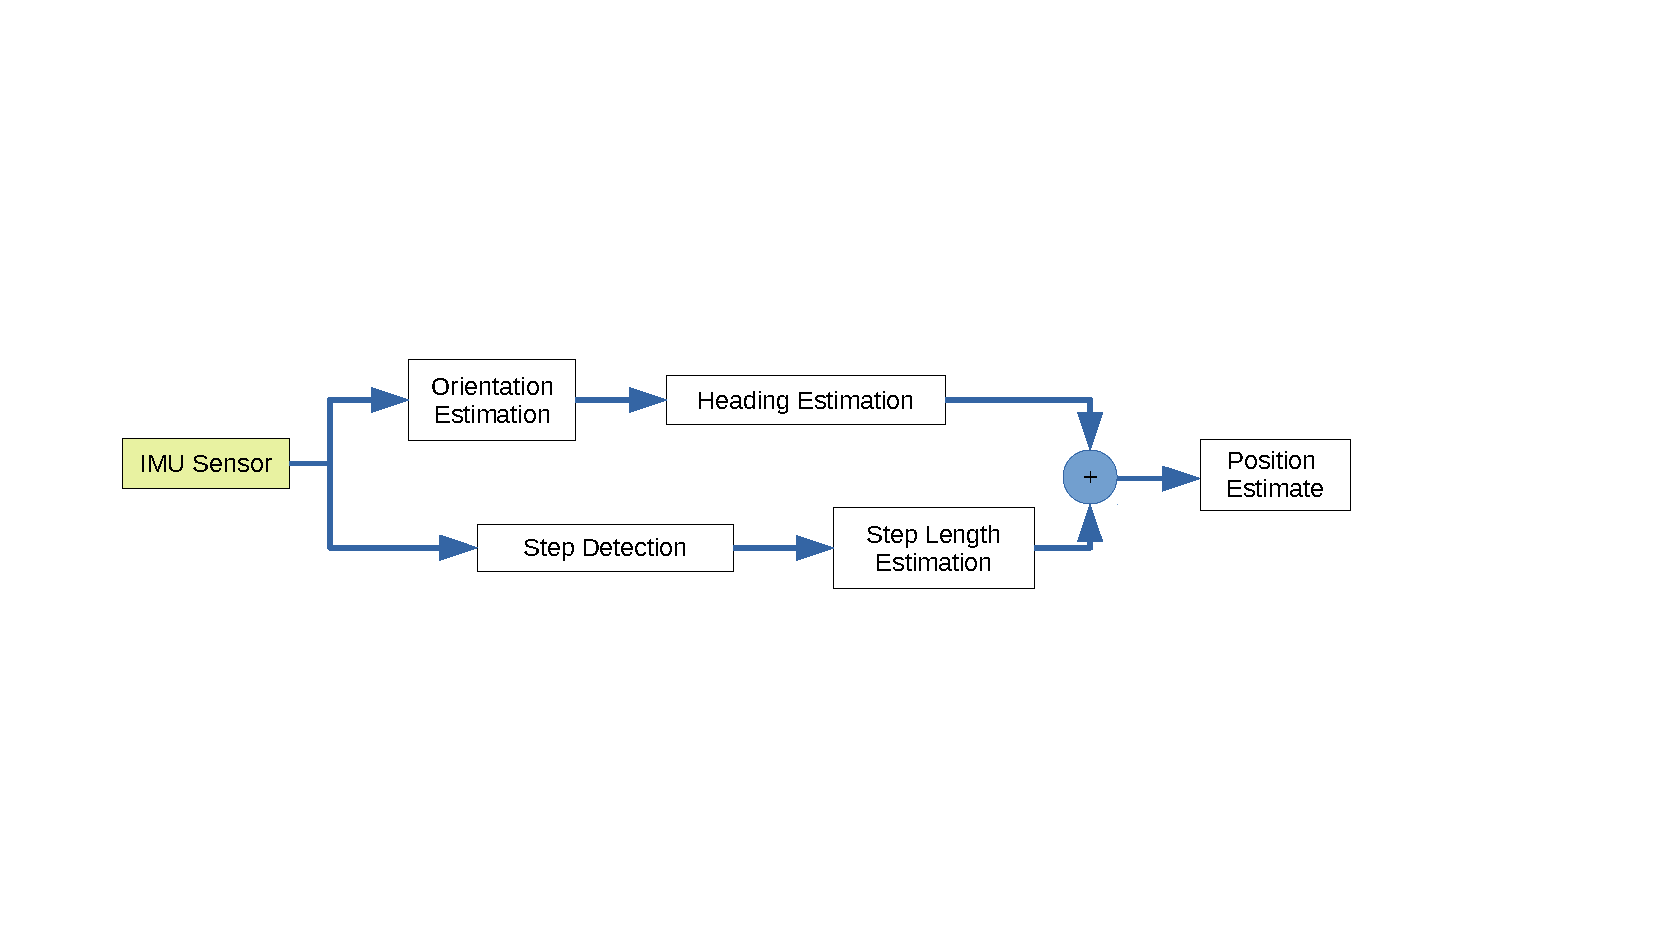
\includegraphics[trim=40 120 180 80, clip,width=\linewidth]{images/shs_diagram}
	\caption{\ac{SHS} pedestrian dead reckoning}
	\label{fig:shs_diagram}
\end{figure}
A step and heading system, as shown in \cref{fig:shs_diagram}, is a form of dead reckoning that detects steps, estimates step length, and the heading in which the pedestrian is moving. This position estimation can be represented by \cite{MunozDiaz2019}
\begin{equation}
	\label{eq:SHS_dynamic_model}
	\left(\begin{array}{l}
		x_t \\
		y_t
	\end{array}\right) 
	=
	\left(\begin{array}{l}
		x_{t-1} \\
		y_{t-1}
	\end{array}\right) 
	+l_{t} \left(\begin{array}{l}
		\cos \left(\theta_{t}\right) \\
		\sin \left(\theta_{t}\right)
	\end{array}\right)
\end{equation}

where $x_{t}$  and  $y_{t}$ represent the position in the $x$-axis and $y$-axis at time  $t$, respectively. $l_{t}$ stands for the step length, while $\theta_{t}$ is the step heading of the pedestrian at time $t$.
Similarly to INS with ZUPT measurement updates, SHS position error is proportional to the number of steps taken. The largest difference is that this error growth does not have a preference of using foot-based sensors, allowing for other sensor placements \cite{Diez2018b}. However, other of sources of error can be introduced due to errors in the detection of steps and their length estimation.  Since other sensor placements are possible, SHS is the PDR technique often used with smartphones as the base for sensing [\qn]. 

%This indicates that this technique is appropriate for further investigation in answering the thesis research questions.\\

%This method can be combined with a particle filter \cite{Koivisto2016, Jackermeier2018}. This allows for more constraints, consequently requiring less particles for localization.
\section{Drift Reduction through Map Information}
PDR methods alone accumulate error with time and are therefore not ideal for long-term pedestrian tracking \cite{Hardegger2012}. Drift reduction methods can be used to try and compensate for this error \cite{MunozDiaz2019a}.  These methods use additional information to restrict the possibilities in which the position estimate can be. One approach is by complement the solution with the infrastructure dependent solutions that require external signal generation \cite{Gu2019}. Another source of information is spatial context \cite{Gu2019}. This includes maps, spatial models and landmarks.

\subsection{Landmark Detection}
A map describes the indoor layout of building, often in the form of of a floor plan \cite{Gu2019}. Using maps assumptions or simplification to restrict the movement. Examples include restricting the movement to be parallel to the outer walls of a building \cite{Abdulrahim2011}. Another is representing the indoor environment as a set of links and nodes, along which the position estimate can move \cite{Davidson2017,Jackermeier2018} 
One approach to drift reduction is through the use of landmark detection. Landmarks are locations with a unique footprint detectable in sensor data. When the user visits a landmark and this is detected, the location of the landmark can be used to calibrate the position estimate of the user, hence compensating drift \cite{Diaz2017}. In addition to drift reduction by position comparison, landmark detection can also be used in determining the user specific parameters of \ac{SHS} online, such as step length estimation parameters \cite{Gu2019,Shang2015}.  Depending on the sensors available, different landmarks become detectable. Examples of landmarks are doors and stairs \cite{Diaz2017,Gu2019,Torok2014}, but also unique magnetic footprints \cite{MunozDiaz2019}, and electromagentic signal footprints \cite{Gu2019}. Some landmarks can be easily determined beforehand, through the use of available building blueprints \cite{Gu2019}. Others can be detected online \cite{Hardegger2012, Hardegger2016}, not requiring a map representation to be available beforehand, using technique such as \ac{SLAM}. 

One form of landmark detection can be done through activity recognition. \\
\textcolor{cyan}{above section can be smoother} \\ \newline
\textcolor{cyan}{ I need to refer to the use of particle filters and that for PDR their use is two fold, landmark detection and absolute position estimate}

\subsubsection{Activity Recognition}
Activity recognition is large research field in which methods span a broad range of complexity, from simple thresholding to the use of deep learning techniques such as neural networks and its many variations \cite{Lima2019}. Even the subset of activity recognition that use IMU sensors does not decrease the amount of possibilities significantly.

%TODO add drear as activity recognition

The choice for a particular activity recognition method is often a trade-off between performance and computational complexity \cite{Bulling2014}. Considering the scope of this thesis, certain constraints can be applied, such as that the system should be able to function on a smartphone and must use comparable sensors to those found in such devices, thus MEMS IMUs. \citet{Shoaib2015} have performed an extensive survey that focuses on the online activity recognition solely using mobile phone sensors and onboard processing. Other metrics such as resource consumption were also presented. 30 papers were found to meet the requirements of the review. Within the review they indicate that most commonly used classification methods include Decision Tree, support vector machine (SVM), K-nearest neighbor (KNN) and Naive Bayes, in descending order. A third of the papers were found to use decision trees. All but 6 of the papers had the training process occurring offline. The classification process takes the method generated offline, and uses it online to classify new activities. The authors refrain from listing any performance measures, such as accuracy or precision, since no direct comparison between the different methods is made. \citet{Ahmad2020} specifically focuses on seeing whether smartphone activity recognition techniques are also applicable to smartwatches, and what parameters, including classifiers, work best. Activities to recognize included walking, up-stairs, down-stairs, running, and jogging. Their results indicated that  Decision Trees, SVM and KNN had around 90 percent accuracy a minor difference. \citet{Shoaib2016} show that combining information from both a smartwatch and smartphone, complex human activity recognition is improved compared to when only a smart watch is used. 

\subsection{Particle Filter}
\label{sec:method-pf}
In order to counter estimate drift,  map information can be used in combination with a Particle Filter. This is a numerical Bayes estimator able to estimate non linear posterior densities, allowing for multimodal distributions \cite{gustafsson2010particle,kihlberg2012map}. Multimodal distribution refers to distributions with multiple maxima in the probability density function. This allows the particle filter to have multiple hypothesis for the system that it is modeling. In the case of localization, it may therefore indicate that there are two position estimates are equally as likely based on the information that the filter has received so far. This can occur due to symmetry in the indoor environment \cite{Woodman2008}. \\
The particle filter is known to work well in three dimensional state space \cite{gustafsson2010particle}, with higher dimensions making the particle representation too sparse to be a meaningfully represent the posterior distribution. Since for indoor localization only y position, x position and heading are needed, the particle filter is sufficient.
\par
As the name suggests, the particle filter uses a finite amount of particles to determine a state estimate. These particles are weighted and are propagated through a motion model, augmented with a noise realization on relevant variables. These noise realizations represent uncertainty of certain components of the motion model. The probability density function of these noise realizations are defined beforehand. Taking the weights of each particle into account a prior estimate can be made. \par 
Measurement updates are used to calibrate the particles throughout their trajectory. These measurements may come from different sources, including map information and landmark detection. When a measurement occurs the particle cloud is compared with the measurements, adjusting the individual weights accordingly. This process is familiar to the reader as it closely resembles that of the previously mentioned Kalman Filter, also a Bayes estimator.\par

\citet{Harle2013} can help limit drift and absolute position estimate

\begin{enumerate}
	\item \textbf{Measurement update} \\
	Each particle is weighted against constraints or system evaluation function. The likelier the particle is within the system constraints, the higher the weighting is. Each particle's weight is redefined through \cref{eq:gen_pf_weight},	where the normalization weight ($c_k$) is given by \cref{eq:gen_pf_probability density}.
	Here $\omega^i_k$ is the weighting for particle $i$ at time $k$, $y_k$ is the measurement at time $k$,  and $N$ is the total number of particles.
	
	\item  \textbf{Estimation} \\
	Using the weightings and positions of the particle cloud, an estimate can be made of the posterior probability density of the process that is being modeled  \cite{gustafsson2010particle}. There are different ways of defining the eventual position estimate. The maximum a posteriori (MAP) estimate picks the particle with the highest weight from the posterior probability function \cite{Saha2009}, while the  minimum mean square error (MMSE) estimate calculates a weighted mean \cite{gustafsson2010particle,Saha2009} as in \cref{eq:gen_pf_estimation}.
	
	\item \textbf{Resampling} \\
	Depending on the new weights of the different particles, a subset is taken and resampled to form a new set of particles, which will be used in the next iteration of the particle filter.
\end{enumerate}

%\begin{algorithm}[H]
%	\SetAlgoLined
%	\caption{Bootstrap Particle Filter}
%	\label{algo:bootstrap_PF}
%	choose the number of particles N.\\
%	% choose a proposal distribution $ q(x_{k+1}|x_{1:k},y_{k+1})$, resampling strategy and the number of particles N.\\
%	% \KwResult{Write here the result }
%	\underline{initialization:}
%	Generate 
%	\begin{subequations}
%		\begin{equation}
%			x^i_1 \sim p_{x_1},
%		\end{equation}
%		and let
%		\begin{equation}
%			\omega^i_{1|0} = 1/N.
%		\end{equation}
%	\end{subequations}
%	\;
%	\For{k = 1,2,...}{
%		\underline{measurement update:}\\
%		\begin{subequations}
%			
%				
%				\begin{equation}
%					\omega^i_{k|k} = \frac{1}{c_k} \omega^i_{k|k-1} p(y_k|x^i_k),
%			\label{eq:gen_pf_weight}	
%			\end{equation}\\
%				where the normalization weight is given by
%				\begin{equation}
%					c_{k}=\sum_{i=1}^{N} w_{k | k-1}^{i} p\left(y_{k} | x_{k}^{i}\right)
%					\label{eq:gen_pf_probability density}
%				\end{equation}
%			
%			\underline{estimation:}\\
%			\begin{equation}
%				\hat{x}_{k | k} =\sum_{i=1}^{N} w_{k}^{i} x_{k}^{i}.
%				\label{eq:gen_pf_estimation}
%			\end{equation}
%			\underline{resampling:}\\
%			take $N$ samples with replacement from the set $\{x^i_{1:k}\}^N_{i=1}$ where the probability to take sample i is $\omega^i_{k|k} = 1/N$.\\
%			\underline{time update:}\\
%			Generate predictions according to the dynamic model, using realizations of the process and measurement noise.
%			\begin{equation}
%				\label{eq:PF_dynamic model}
%				x_{k+1}^{i} \sim p\left(x_{k+1}^{i} | x_{k}^{i}\right)
%			\end{equation}
%		\end{subequations}
%		
%	}
%\end{algorithm}


\section{SHS Components}
\subsection{Walk and Step Detection}
\label{sec:rw - step detection}
Walk detection is determining from sensor data whether a walking activity is being performed. Step detection is deciding when during the walking activity a step is taken. \\
Techniques such as feature classification, frequency domain analysis, and time-domain thresholding can be used to detect the two activities \cite{Yang2014}. An overview of techniques  is  shown in \cref{fig:step_detection_options} and summarized in \cref{tab:step_detection_comparison}. %The reader is referred to \cite{Brajdic2013} for a detailed explanation of each solution.

Naturally, each form of analysis for walk and step detection has its advantages and disadvantages.\\
Time-domain analysis often uses the acceleration norm, making it robust to sensor orientation \cite{Davidson2017}. Its simplest form, thresholding, is trivially simple to implement. The problem with thresholding is that it is difficult to determine the optimal value, as it can vary between users, surfaces, and even shoes \cite{Brajdic2013}. \\
Similar to time-based methods, the periodicity in the norm of acceleration during locomotion is frequently invariant to sensor placement. This therefore also makes frequency analysis robust to sensor orientation. Frequency methods have the disadvantage that they are only able to detect periodic motion. 
For both frequency and time domain-based analysis, it is possible that certain motions, aside from the desired motion, can cross the threshold and generate false positives. In addition, frequency analysis and template matching, a more advanced time based method, will have a certain computational overhead to consider \cite{Davidson2017, Harle2013}. \\
Feature classification methods use features in accelerometer traces to classify steps, using form of machine learning. These method have the advantage that they can determine relations from labeled data automatically, removing a need for humans to define them. This is also a disadvantage as it requires labeled data, the gathering of which can be a labor-intensive process \cite{Bulling2014}. Furthermore, the relationships they determine will depend on the data gathered. This may lead to person dependent performance [\qn]. In addition, certain classification methods may require significant processing power, limiting the platforms on which it can perform [\qn].


\begin{figure}
	\centering
	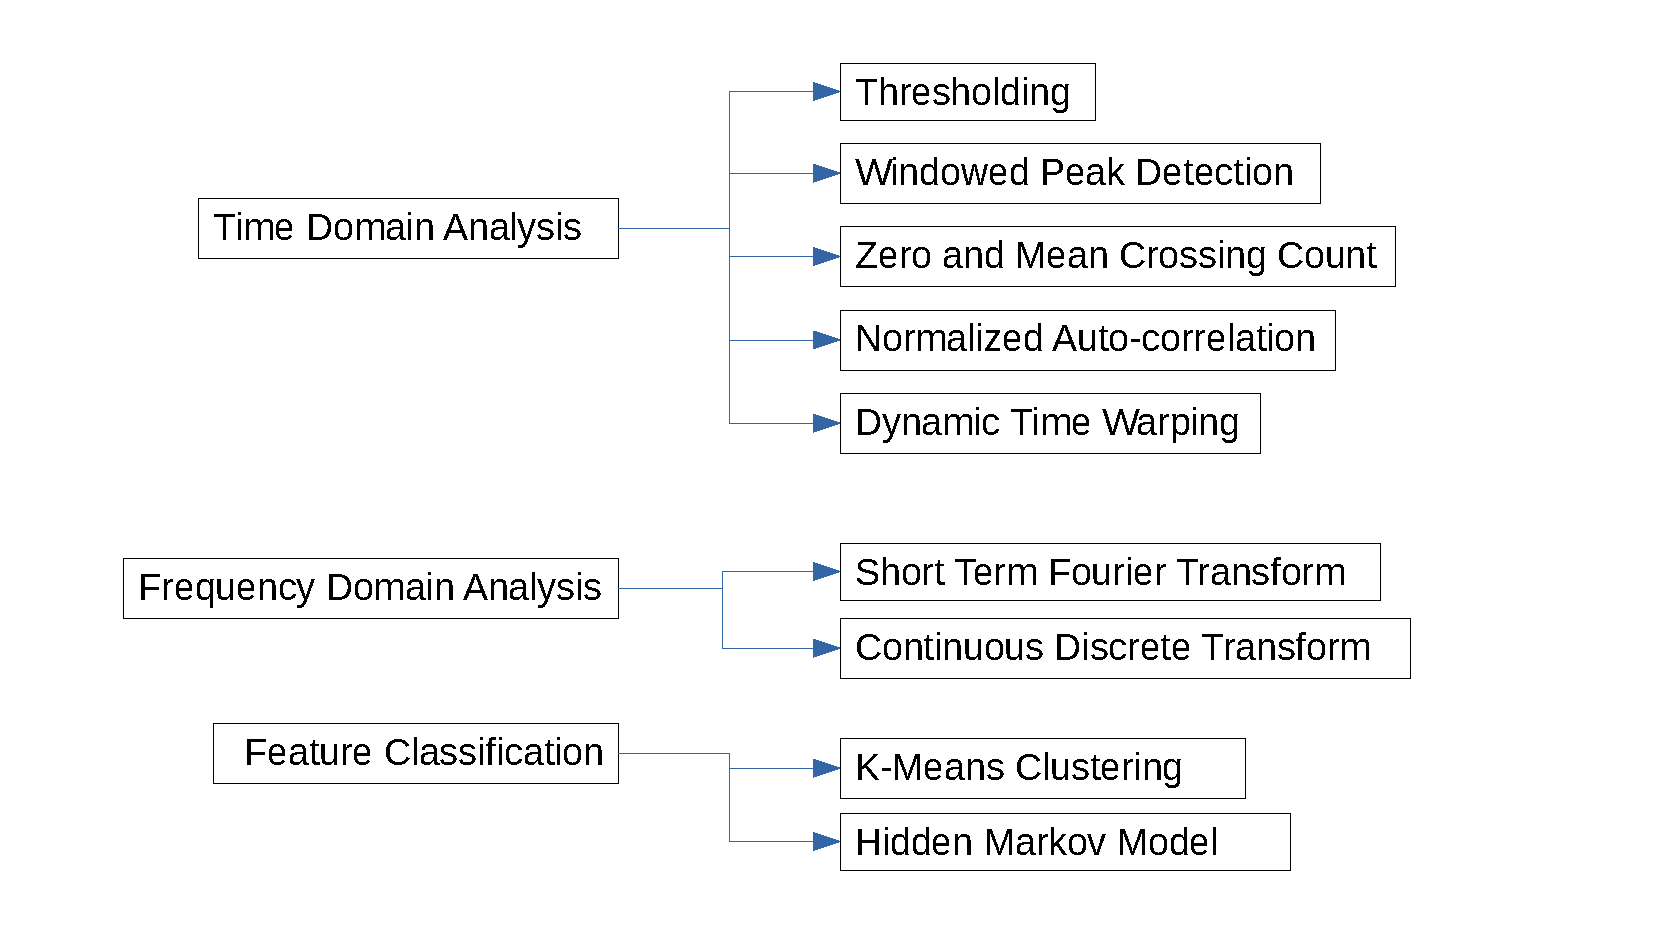
\includegraphics[trim=0 15 0 20, clip,width=0.7\linewidth]{images/step_detection_options}
	\caption{Overview of walk and step detection methods}
	\label{fig:step_detection_options}
\end{figure}

	\begin{table}
	\centering
	\footnotesize
	\begin{tabularx}{\linewidth}{@{} P{17mm} L}
		\toprule
		\thead[lb]{Technique}	&   \thead[c]{Explanation}	\\
		\midrule			
		Threshold & Acceleration magnitude is monitored for the passing of certain values or sign changes, in the case of Zero Crossing method \cite{Davidson2017,Harle2013}. Typically determines when the foot is on the floor \cite{Harle2013}, but has also been applied to pitch angle of the upper leg, where the sensor has been placed \cite{Diaz2014a}. In some instances, the thresholds are altered adaptively, for example through different motion mode detection or information gathered from the previous step \cite{Wu2019}.\\ \cline{1-2}
		(Windowed) Peak Detection & Recognizes local maximum or minimum on acceleration magnitude caused by foot impact on the floor, often within a sliding window \cite{Susi2013}. Generally combined with thresholding, which is one of the simplest combination used with \ac{SHS} \cite{Davidson2017}. \\ \hline
		Auto-correlation (Template Matching) &  Finds correlation of a signal with a time-shifted copy of itself. It leverages the strong cyclic nature of bipedal locomotion \cite{Harle2013}. Since the lag for the highest correlation is not known beforehand, an interval is often swept and correlation values compared. \\ \hline
		Dynamic Time Warping & Similar to autocorrelation, it measures the similarity between two waveforms from accelerometer data \cite{Davidson2017}, These waveforms can both come from the data or one could be a stride template generated offline. A non linear mapping between the two methods is made, resulting in a DTW distance. A smaller distance indicates higher similarity \cite{Davidson2017}.  \\ \hline
		Short Term Fourier Transform & Transforms acceleration signal of successive windows of data into the frequency domain. For spectral analysis, a subset containing a stride (two steps) is required to determine the frequency \cite{Harle2013}.  \\ \hline
		Wavelet Decomposition & Acceleration magnitude is split into low and high-frequency components, from which the dominant frequency is assumed to be the walking frequency. Iterating this process on the resulting low-frequency signal approximation, a smoother shaped dominant low-frequency signal is generated. The frequency of this signal corresponds to walking cadence \cite{Davidson2017}. \\ \hline	
		Hidden Markov Model & Uses gait cycles segmented into different states of a state machine, to determine if a step has been taken \cite{Ren2016a}. Thresholds can be used to induce a state change. If a full state machine cycle is achieved, a step is detected.\\ \hline
		K Nearest Neighbours & Uses labeled data containing features from successive time windows and compares a new time window with its features. It finds the labeled data whose features are most similar. This new set then recieves its label. \\
		\bottomrule
	\end{tabularx}
	\caption{Overview of different step detection methods}
	\label{tab:step_detection_comparison}
\end{table}

In \cite{Brajdic2013}, a variety of algorithms for both walk detection and step detection on unconstrained smartphones are tested and compared. The paper reviews techniques with different levels of complexity from a variety of different papers. In order to compare the different techniques, \citet{Brajdic2013} collected a large dataset from 27 test subjects leading to 130 recordings was made. Each subject held the smartphone in six different carrying modes: in hand in front of user (idle and with device interaction), in a front pocket, in a back pocket and in a handbag or backpack. A ground truth was generated by video recording each session and manually counting the amount of steps taken. Using this dataset a comparison is made between the nine algorithms.
\newline
The paper concludes that for the generated dataset, the best step counting results were obtained using the windowed peak detection, hidden Markov model, and continuous wavelet transform. Each had a median error of about 1.3\%.\\
Considering the relative simplicity of the technique, the authors recommend that windowed peak detection as the most efficient algorithm for step detection. The best walk detection algorithms were thresholds on either standard deviation or signal energy,  short-term Fourier transform, and normalized autocorrelation.\\
\citet{Salvi2018} build upon the conclusions and recommendations of \citet{Brajdic2013}, with the aim of further optimizing the windowed peak detection algorithm and its parameters. The algorithm is based on the approach of \citet{Palshikar2009} and consists of 5 stages run in series. These are pre-processing, filtering, scoring, detection and post processing. An exhaustive grid search across the parameter space was performed to find the optimal set for step detection. Using these parameters, an average accuracy of $95\% \pm 4.5\%$ was reached for the different carrying modes. 

%These results make this approach 


\subsubsection{Step Length Estimation}
In order to generate a displacement vector from step detection, the step length must be estimated. \citet{Collins2013a} found that increasing step speed leads to larger step lengths, while step speed can have slow and spontaneous fluctuations depending on the motion mode. In addition, step size depends on the physical characteristics of the user and on their walk strategy, which can be different per individual \cite{Diez2018}. These discrepancies indicate that using a simple average step length for every pedestrian could result in quick accumulation of error. 

\citet{Diez2018} categorizes step length estimation methods into integration based and model-based methods. \\
Theoretically, the double integration of the IMU acceleration signal is the best approach to step size estimation, using the INS approaches outlined in chapter \secref{sec:INS}. This would give a direct measurement of displacement. It does not require any modeling, assumptions, or person-specific calibration \cite{Diez2018}. However, since it would be an INS approach, it suffers from the same drift problems and would require the same solutions. Therefore this approach benefits from having the sensor to be located on the foot. \\
Analytical models can be made of human mobility based on geometrical relationships of body composition, angles, and displacement of body parts. One of the largest disadvantages of a model-based approach is that human proportions are not uniform, requiring approximations and/or some form of calibration for the model to be accurate.
An overview of different step length estimation methods can be found in \cref{tab:step_length_methods}.

\begin{table}[H]
	\centering
	\textcolor{cyan}{Table with different step length methods}
	\caption{Different Step Length Methods}
	\label{tab:step_length_methods}
\end{table}

\citet{Vezocnik2019} compared different existing step length estimation algorithms. The review focuses on the methods applicable to smartphone use. This means methods that do not require training and do not require the sensor to be placed on the foot. This, therefore, excludes machine learning and INS systems. The models used are either based on an inverted pendulum model or relate predictors to step length. Examples of step length predictors are step frequency and acceleration range within a step. The robustness of the methods was tested by having the smartphone in different carrying modes. This includes front 

\begin{equation}
	\label{eq:Tian2016_sle}
	\text{step size} = K \cdot h \cdot \sqrt{F}.
\end{equation}

Here $K$ is a tunable parameter, $h$ is the height of the user and $F$ is the step frequency. This method reported an average error of  4.59 \% for personalized variables and 6.96 \% for global ones. For personally tuned variables the method of \cite{Weinberg2002} was best. This is an inverted pendulum model in which the human center of mass is used, located approximately at the pelvis. The center of mass rotates as an inverted pendulum when taking a step. This is followed by a forward horizontal displacement when both feet are on the ground \cite{Diez2018}. The model is defined as 

\begin{equation}
\text{step size} =K \sqrt[4]{A_{\max }-A_{\min }}.
\label{eq:weinberg_stepsize}
\end{equation}

Here $A_{\max}$ is the largest measured acceleration measured within a step interval, while $A_{\min}$ is the smallest. $K$ is a calibration variable  \cite{Weinberg2002,Diez2018}. The model had an average error of  10.64 \% for global variables and  3.60 \% for personalized \cite{Vezocnik2019}.



\subsubsection{Step Heading Estimation}
Step heading determines the direction of a detected step. It requires the orientation of the sensor in the navigation frame and determining in what direction the sensor is moving in the sensor frame. This provides an estimate in which direction the sensor is moving in the navigation frame.  Step heading estimation is currently the component within SHS whose performance is the most limiting for positioning purposes \cite{Diez2018b, Qian2013,Combettes2017}.\\
Even though the phone orientation may be known accurately, the direction in which the user is moving is not instantly clear. \par
There are two approaches to determining the heading. The first is knowing beforehand what the orientation of the phone is with respect to heading \cite{Tian2016}.  This would constrain the carrying mode that can be used.  With the use of motion classification, this method could be expanded, where different carrying modes can be sensed,which changes the heading accordingly. Heading per carrying mode would need to be derived beforehand, through the training of the necessary model. 

\textcolor{cyan}{this section is not done yet, and so will need completing } \\ \newline
\textcolor{red}{I do not have a comparison of different orientation estimation methods. How do I explain the use of EKF compared to the different possibilities? Should i just add this comparison section?}

\subsubsection{Activity Recognition}





% The Beauregard implementation introduced backtracking, whereby the filter kept a limited history of each particle’s ancestors to allow deletion of an entire trajectory when a particle was killed due to a wall constraint. This is a variant of backward belief propagation also used by Rai et al. [23] and is useful to improve position estimates made in the past when live positioning is not a requirement.
